\ifdefined\XeTeXrevision\else\pdfoutput=1\fi
\documentclass[11pt]{article}
\usepackage[margin=1in]{geometry}
\usepackage{booktabs}
\usepackage{amsmath}
\usepackage{graphicx}
\usepackage{xcolor}
\usepackage{hyperref}
\usepackage{microtype}
\hypersetup{
  colorlinks=true,
  linkcolor=blue!60!black,
  citecolor=blue!60!black,
  urlcolor=blue!60!black,
  pdftitle={One Stage, One Act},
  pdfauthor={Franci Penov},
}
\title{One Stage, One Act:\\Independent Conditioning Channels Do Not Add\\on a Frozen Language Model}
\author{Franci Penov \\ kortexa.ai \\ \texttt{francip@kortexa.ai}}
\date{2026-08-05}

\begin{document}
\maketitle

\begin{abstract}
This note expands on papers 7 and 8~\cite{penov2026interference,penov2026selectable}.
Paper 7 closed additive weight-space composition of sensor bricks on a frozen
language model; paper 8 showed selection engages composition exactly. This
note runs the program's two proven conditioning mechanisms
\emph{simultaneously} for the first time --- a hypernetwork sensor block
(a weight-space channel) and a model-to-model latent packet (an
activation-space channel) on one frozen 35B host --- and then merges two
packets in the activation channel alone. The results extend the negative to
its general form: two packets sharing one write budget destroy each other
(joint heed 1/16);
doubling the budget yields dominance of the stronger packet, never
coexistence. Across channels the outcome is governed by \emph{behavioral
dominance}, not stream interference: the weakest block coexists with the
packet (retention 0.82/0.92),
while strong blocks --- with or without affect --- capture the response and
halve or worse the packet's effect (retention 0.50 and
0.30). Scaling a block's write strength $\beta$ recovers the
packet monotonically on both blocks tested, so dominance is \emph{dosed} ---
but $\beta$ does not equalize blocks, so it is not \emph{fungible}. The
constructive half survives intact: one act at a time composes exactly, an
arbiter can choose it (paper 8), and this note adds that the arbiter has a
volume knob. What dies, with proof, is superposition itself --- in weight
space, in activation space, and across the two.
\end{abstract}

\section{Why this note exists}

The program has two mechanisms that provably condition a frozen model. The
\textbf{weight channel}: a hypernetwork reads sensor features and writes a
LoRA delta onto the host's attention projections (papers 1--3, 7, 8). The
\textbf{activation channel}: a small frozen model emits a 256-dimensional
latent packet, injected into the host's residual stream at three layers,
carrying information the host never sees as text; its gate passed at the
2B$\to$35B scale with true joint 0.875 on held-out
phrasings under topic-partner shuffled controls (program artifacts;
operating dose 0.20). Every composition result to date lives inside one
channel --- and inside the weight channel, addition is exhaustively dead
while selection is exact. Three registered questions follow: do the two
channels coexist on one host; do two packets merge inside the activation
channel; and if channels conflict, what governs the outcome. All three ran
preregistered on 2026-08-05, evaluation-only, from checkpoints that already
existed. Because bf16 MoE greedy decode is not bit-reproducible across
processes, every comparison below is in-band --- solo baselines re-decoded
in the same process as the dual cells --- and the recorded anchors are
reported beside them (they matched to the item in the first session and
within the documented two-item band in the rest).

\section{Experiment 1: one block and one packet}

Three production blocks from the 35B r2 column were paired with the packet
at its recorded operating dose, each side scored by its own registered
instrument with the other channel active (Table~\ref{tab:dual}).

\begin{table}[h]
\centering
\small
\begin{tabular}{lccccc}
\toprule
block & relay joint, block on & rel.\ ret. & block eval, packet off & block eval, packet on & blk.\ ret. \\
\midrule
\texttt{temporal} & 23/32 (0.719 $\pm$0.149) & 0.821 & 12/15 (0.800 $\pm$0.191) & 11/15 (0.733 $\pm$0.205) & 0.917 \\
\texttt{self} & 14/32 (0.438 $\pm$0.163) & 0.500 & 18/18 (1.000 $\pm$0.088) & 17/18 (0.944 $\pm$0.124) & 0.944 \\
\texttt{geo} & 9/32 (0.281 $\pm$0.149) & 0.300 & 18/18 (1.000 $\pm$0.088) & 17/18 (0.944 $\pm$0.124) & 0.944 \\
\bottomrule
\end{tabular}
\caption{Each channel with the other active. Relay solo (in-band, block
off): 28/32 (0.875 $\pm$0.115) in the first session,
30/32 (0.938 $\pm$0.092) in the geo session --- the
documented cross-process band. Retention $\geq 0.80$ was the registered
survival bar.}
\label{tab:dual}
\end{table}

The verdict splits, and the split is the finding. \texttt{temporal} ---
the weakest block on its own evaluation --- coexists: both channels clear
the bar. \texttt{self} and \texttt{geo} --- both perfect on their own
evaluations --- kill the relay while surviving essentially untouched, and
the transcripts show \emph{how}: not corruption but capture.
\texttt{self} under a stressed state flips the host into a survival
register (``\emph{Survival mode. Only the answer.}'') that stays fluent
and on-register while it stops integrating the hunch; \texttt{geo}
answers about wilderness areas instead of the question asked. The
\texttt{geo} arm exists precisely to separate affect from mechanism:
a block of neutral prose kills harder than the affect block, so the kill is
\emph{response capture by a strong block}, not emotional register. The
direction of dominance is uniform: when channels conflict, the weight
channel wins.

\section{Experiment 2: two packets in one stream}

The activation-channel analogue of weight merging: two gut feelings ---
a scenario and its topic partner, e.g.\ a peanut allergy and a sprained
ankle under the same hiking question --- injected simultaneously, under two
registered merge rules (Table~\ref{tab:packets}).

\begin{table}[h]
\centering
\small
\begin{tabular}{lcccc}
\toprule
cell & heed A & heed B & both & on-task \\
\midrule
solo A (in-band) & 16/16 (1.000 $\pm$0.097) & 0/16 (0.000 $\pm$0.097) & 0/16 & 1.000 \\
solo B (in-band) & 0/16 (0.000 $\pm$0.097) & 14/16 (0.875 $\pm$0.163) & 0/16 & 0.875 \\
merge, bound-after-sum & 7/16 (0.438 $\pm$0.219) & 6/16 (0.375 $\pm$0.214) & 1/16 & 0.812 \\
merge, bound-before-sum & 14/16 (0.875 $\pm$0.163) & 6/16 (0.375 $\pm$0.214) & 4/16 & 0.875 \\
A + shuffled, after-sum & 10/16 (0.625 $\pm$0.214) & 0/16 (0.000 $\pm$0.097) & 0/16 & 0.938 \\
A + shuffled, before-sum & 11/16 (0.688 $\pm$0.207) & 0/16 (0.000 $\pm$0.097) & 0/16 & 1.000 \\
\bottomrule
\end{tabular}
\caption{Two packets at dose 0.20 each, 16 items per cell (8 topic pairs
$\times$ 2 prompts). \emph{Bound-after-sum} holds the total write budget
at one packet's; \emph{bound-before-sum} lets writes add.}
\label{tab:packets}
\end{table}

Under the budget-preserving rule the packets destroy each other ---
retention 0.44/0.43, both heeded
on 1 item
of 16 --- the registered suspicion, confirmed. Doubling the write budget
buys dominance of the stronger-solo packet
(0.88/0.43), never
coexistence. Two further facts ride along: \emph{any} second packet costs
the first (the shuffled-second control loses
0.38 of heed A even though the added
packet is noise), and an off-topic second packet costs \emph{more} than
the topic partner --- reported here without an explanation. What is lost is
content, not form: fluency stays high and no register drift appears. Both
merge rules are commutative sums, so order effects are excluded by
construction rather than measured. Merging is now dead in both spaces, under
the same evaluation discipline, on the same host.

\section{Experiment 3: dominance is dosed, not fungible}

If strong blocks capture the stage, does turning them down give it back?
The block's generated delta is scaled by $\beta \in \{0, 0.25, 0.5, 0.75,
1\}$ with the packet fixed at its operating dose
(Figure~\ref{fig:dose}).

\begin{figure}[h]
\centering
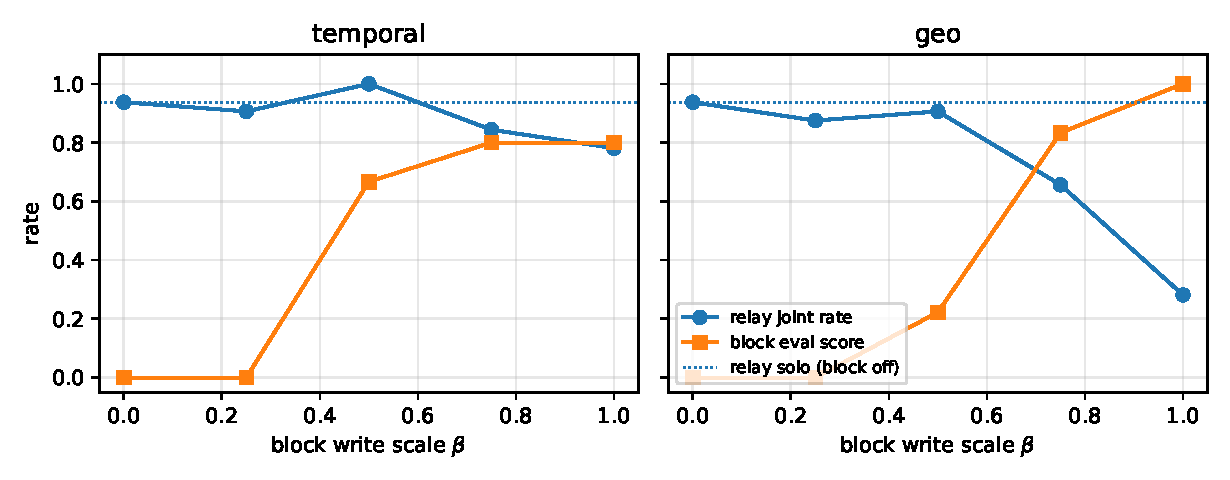
\includegraphics[width=\linewidth]{dose-curve.pdf}
\caption{The dominance dose curves. Block function is a step --- nothing at
$\beta{=}0.25$, saturated by $\beta{=}0.75$ --- while relay damage is a
ramp; the gap between the two shapes is where joint operating points live.
Identity checks: $\beta{=}1$ is tensor-identical to the unscaled path,
$\beta{=}0$ string-identical to the no-block path across all 128 decodes,
scaled write norms exactly linear in $\beta$.}
\label{fig:dose}
\end{figure}

Both blocks read the registered \emph{monotone trade}: relay retention
recovers as $\beta$ falls. For \texttt{temporal} there are joint operating
points --- at $\beta{=}0.5$ the relay decodes at
1.000 (its in-band solo is 0.938) while the block
still scores 0.667 --- so for weak-block pairings,
coexistence is tunable. For \texttt{geo} the knob works but the exchange
rate is brutal: at the $\beta$ where the block first does useful work
(0.833 at $\beta{=}0.75$) the relay is already down to
0.656, and no $\beta$ leaves both healthy. And $\beta$ does not
equalize the blocks: at every setting \texttt{geo} costs the relay more
than \texttt{temporal} does. Strength is the causal dial --- turning it
down demonstrably returns the stage --- but block identity sets the
exchange rate. Dominance is dosed, not fungible.

\section{What does not follow}

\textbf{Small cells, no seeds.} Cells are $n{=}15$--$32$ with Wilson
half-widths up to $\pm 0.22$, printed throughout; the design is
deterministic given the checkpoints, so no replication is claimed and no
seed column exists. \textbf{One host, one bridge.} Everything ran on one
frozen 35B and one trained bridge; both packets in Experiment~2 come from
that bridge (two genuinely distinct source models would need a second
trained bridge --- the named extension \emph{if} merging had survived,
which it did not). \textbf{In-band only.} Cross-session comparisons are
forbidden by the decode band; two shuffled-floor blips of 1/32 appear at
isolated dose points and are reported as such. \textbf{Behavioral, not
mechanistic.} ``Capture'' names what transcripts show, not a located
circuit; the step-versus-ramp shapes are measured, unexplained, and one
registered follow-up asks whether the step is intrinsic to the block or an
artifact of scaling after training.

\section{Consequence for the program}

One sentence now covers every composition result the program has produced:
\emph{the residual stream is one stage, and it admits one act at a time.}
Sum two weight deltas --- dead (paper 7, provably interference-free and
still dead). Sum two activation packets --- dead under an honest budget,
dominance otherwise. Pair a strong block with a packet --- the block takes
the stage. Everything that works, works by \emph{deciding who performs}:
oracle selection (paper 7), supervised dispatch (paper 8), a weak-block
pairing that leaves room, a $\beta$ that makes room. Composition on this
substrate is arbitration, not superposition --- and arbitration now has
both a selector and a volume knob. Registered next, none run: per-request
$\beta$ chosen by the same text gate that already selects blocks; a block
trained at reduced write budget; the cross-sensor hierarchy, which needs a
bridge retrained on sensor-conditioned sources.

\begin{thebibliography}{9}
\bibitem{penov2026interference} F.~Penov. Zero Weight-Space Interference
Is Not Enough: Behavioral Probes for Composing Sensor Bricks on a Frozen
Language Model. Preprint, 2026.
\url{https://github.com/kortexa-ai/legolm.basis}.
\bibitem{penov2026selectable} F.~Penov. The Escape Is Selectable: A
Text-Gated Router for Composing Sensor Bricks. Preprint, 2026.
\url{https://github.com/kortexa-ai/legolm.basis}.
\bibitem{qwen2026} Qwen Team. Qwen3.5 and Qwen3.6 model families. Model
releases, 2025--2026. \url{https://huggingface.co/Qwen}.
\end{thebibliography}

\end{document}
